\chapter{控制系统的时域分析与综合}
\section{典型输入信号}
\begin{definition}[单位阶跃函数]
    单位阶跃函数的表达式如下：
    \begin{equation*}
        r(t) = \begin{cases}
            1 \quad & t\geq 0 \\
            0 \quad & t<0
        \end{cases}
    \end{equation*}
    示意图如图：
    \begin{center}
        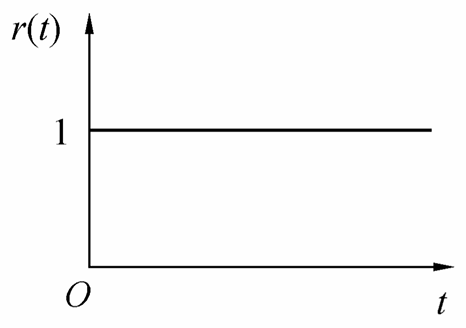
\includegraphics[width=.2\textwidth]{note/time-domain analysis/figure/1.png}
    \end{center}
    Laplace变换后：$R(s) = \dfrac{1}{s}$
\end{definition}

\begin{definition}[单位斜坡函数]
    单位斜坡函数的表达式如下：
    \begin{equation*}
        r(t) = \begin{cases}
            t \quad & t>0 \\
            0 \quad & t<0
        \end{cases}
    \end{equation*}
    示意图如图：
    \begin{center}
        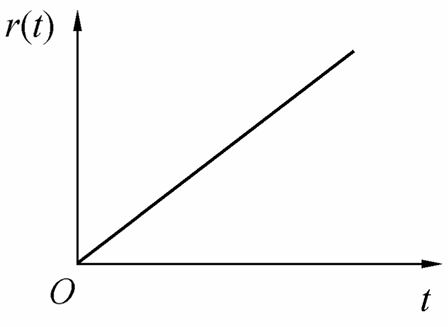
\includegraphics[width=.2\textwidth]{note/time-domain analysis/figure/2.png}
    \end{center}
    Laplace变换后：$R(s) = \dfrac{1}{s^2}$
\end{definition}

\begin{definition}[单位加速度函数]
    单位加速度函数的表达式如下：
    \begin{equation*}
        r(t) = \begin{cases}
            \frac{1}{2}t^2 \quad & t\geq 0 \\
            0 \quad & t<0
        \end{cases}
    \end{equation*}
    示意图如图：
    \begin{center}
        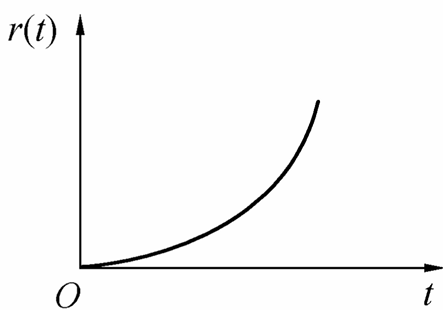
\includegraphics[width=.2\textwidth]{note/time-domain analysis/figure/3.png}
    \end{center}
    Laplace变换后：$R(s) = \dfrac{1}{s^3}$
\end{definition}

\begin{definition}[单位冲激函数]
    单位冲激函数的表达式如下：
    \begin{equation*}
        \begin{split}
            &\delta(t) = \begin{cases}
                \infty \quad & t\neq 0 \\
                0 \quad & t=0
            \end{cases}\\
            &\int_{-\infty}^{\infty} \delta(t) dt = 1
        \end{split}
    \end{equation*}
    Laplace变换后：$R(s) = 1$
\end{definition}

\begin{definition}[正弦信号]
    正弦信号的表达式如下：
    \begin{equation*}
        r(t) = A \sin (\omega t + \varphi)
    \end{equation*}
    Laplace变换后：$R(s) = A e^{\frac{\varphi}{\omega} s} \dfrac{\omega}{s^2+\omega^2}$
\end{definition}

\begin{definition}[动态性能指标]
    在时域分析中我们主要关注以下几个动态性能指标：
    \begin{enumerate}
        \item 延迟时间$t_d$：系统响应从0第一次上升到稳态值的50\%所需要的时间
        \item 上升时间$t_r$：
        \begin{itemize}
            \item 有振荡系统时：系统响应从0第一次上升到稳态值所需的时间
            \item 无振荡系统时：系统响应从稳态值的10\%上升到90\%所需的时间
        \end{itemize}
        \item 峰值时间$t_p$：系统响应第一次达到最大峰值所需要的时间
        \item 超调量$\sigma$：系统响应超出稳态值的最大偏移量（常以百分比表示），$\sigma\% \triangleq \dfrac{y(t_p) - y(\infty)}{y(\infty)}$
        \item 调节时间$t_s$：系统响应与稳态值之差达到并维持误差$\pm\delta$所需要的最短时间，即：$\left\lvert\dfrac{y(t_p) - y(\infty)}{y(\infty)} \right\rvert \leq \delta ,t\geq t_s $
        \item 震荡次数$N$：调节时间$t_s$内，$y(t)$偏离$y(\infty)$的振荡次数
    \end{enumerate}
\end{definition}

\section{一阶系统的时域分析}
\subsection{一阶系统的单位阶跃响应}
\begin{enumerate}
    \item 输入量：$r(t) = 1$ ，$R(s) = \dfrac{1}{s}$
    \item 输出量：$Y(s) = G(s)R(s) = \dfrac{1} {(Ts+1)s}$ ， $y(t) = 1- e^{-\frac{t}{T}}$
    \item 延迟时间：$t_d = 0.69T$
    \item 上升时间：$t_r = 2.2T$ 
    \item 调节时间：$t_s = 3T \,(\Delta = 5\%)$
\end{enumerate}

\begin{ascolorbox3}{一阶系统单位阶跃响应特点}[color = red!40!yellow][coltitle=blue!50!green]
    \begin{enumerate}
        \item 系统输出为初值为0，终值为1的单调连续上升过程。
        \item 响应曲线终值为1，稳态误差为0。
        \item 响应曲线在$T=0$时斜率最大，为$\dfrac{1}{T}$
        \item 动态性能与常数$T$有关，当$t=T$时，响应曲线上升到稳态值的63.2\%
    \end{enumerate}
\end{ascolorbox3}

\subsection{一阶系统的单位冲激响应}
\begin{enumerate}
    \item 输入量：$r(t) = \delta(t)$，$R(s) = 1$ 
    \item 输出量：$Y(s) = \dfrac{1}{Ts+1}$，$y(t) = \dfrac{1}{T} e^{-\frac{t}{T}}$
\end{enumerate}

\begin{ascolorbox3}{一阶系统单位冲激响应特点}[color = green!40!blue][coltitle = red!60!yellow]
    \begin{enumerate}
        \item 系统输出时单调连续下降的指数曲线
        \item 响应曲线的终值为0，稳态误差为0
        \item 动态性能与常数$T$有关，$y(0) = \dfrac{1}{T}\quad y(T) = 0.368\dfrac{1}{T}\quad y(\infty) = 0$
        \item 和传递函数一样，单位冲激响应可以反映系统全部性质，单位冲激响应与传递函数互为Laplace变换对
    \end{enumerate}
\end{ascolorbox3}

\subsection{一阶系统的单位斜坡响应}
\begin{enumerate}
    \item 输入$r(t) = t$，$R(s) = \dfrac{1}{s^2}$
    \item 输出$Y(s) = \dfrac{1}{s^2(Ts+1)}$，$y(t) = t-T(1-e^{-\frac{t}{T}})$
    \item 误差量：$e(t) = T(1-e^{-\frac{t}{T}})$，$e(\infty) = T$
\end{enumerate}

\section{二阶系统的时域分析}
\begin{definition}[二阶系统的标准形式]
    标准形式的二阶系统满足以下式子：
    \begin{enumerate}
        \item 开环传递函数：$G(s) = \dfrac{\omega_n^2}{s(s+2\zeta \omega)}$
        \item 闭环传递函数：$\varPhi(s) = \dfrac{\omega_n^2}{s^2 + 2\zeta \omega_n s + \omega_n^2}$
        \item 闭环极点：$s_{1,2} = -\zeta \omega_n \pm \omega_n \sqrt{\zeta^2 -1}$
    \end{enumerate}
    其中$\omega_n$为无阻尼振荡频率，$\zeta$为阻尼比
\end{definition}

\subsection{二阶系统的单位阶跃响应}
根据$\zeta$的取值我们可以把响应分为四种情况：欠阻尼、零阻尼、过阻尼、临界阻尼和负阻尼

\subsubsection{欠阻尼情况$(0<\zeta<1)$}
欠阻尼条件下$\zeta$满足$0<\zeta<1$，定义阻尼振荡频率：$\omega_d = \omega_n\sqrt{1-\zeta^2}$，则有：
\begin{equation*}
    \begin{split}
        Y(s) &= \frac{\omega_n^2}{s^2 + 2\zeta\omega_n s +\omega_n^2}\cdot\frac{1}{s} = \frac{1}{s} - \frac{s+\zeta \omega_n}{(s+\zeta \omega_n)^2+\omega_d^2}-\frac{\zeta\omega_n}{(s+\zeta \omega_n)^2+\omega_d^2} \\
        y(t) &= \Lcal^{-1}[Y(s)] = 1-e^{-\zeta \omega_n t}(\cos \omega_d t +\frac{\zeta}{\sqrt{1-\zeta^2}} \sin \omega_d t) = 1- e^{-\zeta \omega_n t}\frac{1}{\sqrt{1-\zeta^2}}\sin (\omega_d t +\theta)
    \end{split}
\end{equation*}

\begin{ascolorbox9}{欠阻尼的动态过程指标}
    \begin{enumerate}
        \item 上升时间$t_r = \dfrac{\pi - \theta}{\omega_n \sqrt{1-\zeta^2}}$
        \item 峰值时间$t_p = \dfrac{\pi}{\omega_d} = \dfrac{\pi}{\omega_n \sqrt{1-\zeta^2}}$
        \item 超调量$\sigma_p = e^{-\frac{\zeta}{\sqrt{1-\zeta^2}}\pi} \times 100\%$
        \item 调整时间$t_s = \dfrac{1}{\zeta \omega_n} \ln\dfrac{1}{\Delta \sqrt{1-\zeta^2}}\text{(近似解)} = 
        \begin{cases}
            \dfrac{4}{\zeta \omega_n} & \quad \Delta = 0.02 \\
            \dfrac{3}{\zeta\omega_n} & \quad  \Delta = 0.05 
        \end{cases}\text{（数值解）}$
        \item 振荡次数$N = \begin{cases}
            \dfrac{2\sqrt{1-\zeta^2}}{\pi \zeta} & \quad \Delta = 0.02 \\
            \dfrac{1.5\sqrt{1-\zeta^2}}{\pi \zeta} & \quad \Delta = 0.05
        \end{cases}$
    \end{enumerate}
\end{ascolorbox9}

\begin{example}
    已知二阶系统的闭环传递函数为：
    \begin{equation*}
        \varPhi(s) = \frac{\omega_n^2}{s^2 + 2\zeta \omega_n s +\omega_n^2}
    \end{equation*}
    其中$\zeta = 0.6 \quad \omega_n = 5$rad/s。试计算该系统的单位阶跃响应的特征量$t_r,t_p,t_s,\sigma_p$和$N$\\
    \textbf{解}: 由已知可得：
    \begin{equation*}
        \begin{split}
            t_r/\mathrm{s} &= \frac{\pi-\theta}{\omega_n\sqrt{1-\zeta^2}} = 0.55 \\
            t_p/\mathrm{s} &= \frac{\pi}{\omega_n\sqrt{1-\zeta^2}} = 0.785 \\
            \sigma_p &= e^{-\frac{\zeta \pi}{\sqrt{1-\zeta^2}}}\times 100\% = 9.5\% \\
            t_s/\mathrm{s} &= \frac{4}{\zeta \omega_n} \approx 1.4 \quad \Delta = 0.02\\
            t_s/\mathrm{s} &= \frac{3}{\zeta \omega_n} \approx 1.1 \quad \Delta = 0.05 \\
            N/\text{次} &= \frac{2\sqrt{1-\zeta^2}}{\pi \zeta} \approx 1
        \end{split}
    \end{equation*}
\end{example}

\subsubsection{零阻尼情况$(\zeta=0)$}
在欠阻尼条件下令$\zeta \rightarrow 0$即可得到：
\begin{equation*}
    y(t) = 1- \cos \omega_n t
\end{equation*}

\subsubsection{临界阻尼情况$(\zeta = 1)$}
由已知可以得到系统的响应为：
\begin{equation*}
    \begin{split}
        Y(s) &= \frac{\omega_n^2}{(s+\omega_n)^2}\cdot \frac{1}{s} = \frac{1}{s}-\frac{\omega_n}{(s+\omega_n)^2}-\frac{1}{s+\omega_n}\\
        y(t) &= 1-e^{-\omega_n t}(1+\omega_n t)
    \end{split}
\end{equation*}

\subsubsection{过阻尼情况$(\zeta>1)$}
由已知可以得到系统的响应为：
\begin{equation*}
    \begin{split}
        Y(s) &= \frac{\omega_n^2}{(s+\zeta\omega_n + \omega_n\sqrt{\zeta^2 - 1})(s+\zeta\omega_n - \omega_n\sqrt{\zeta^2 - 1})} \cdot \frac{1}{s} \\
        y(t) &= 1- \frac{1}{2\sqrt{\zeta - 1}(\zeta - \sqrt{\zeta^2 -1})} e^{-(\zeta - \sqrt{\zeta - 1})\omega_n t} + \frac{1}{2\sqrt{\zeta^2 - 1}(\zeta + \sqrt{\zeta ^2 -1})} e^{-(\zeta + \sqrt{\zeta^2 - 1})\omega_n t}
    \end{split}
\end{equation*}

\subsubsection{负阻尼$(-1<\zeta<0)$}
由已知可以得到系统的响应为：
\begin{equation*}
    y(t) = 1 - \frac{e^{-\zeta \omega_n t}}{\sqrt{1-\zeta^2}}\sin (\omega_d t +\theta)
\end{equation*}\\
其中$\omega_d = \omega_n \sqrt{1-\zeta^2} \quad \theta = \arctan \dfrac{\sqrt{1-\zeta^2}}{\zeta}<0$ \\

下图可以同时表现出五种阶跃响应状态之间的变化情况：
\begin{center}
    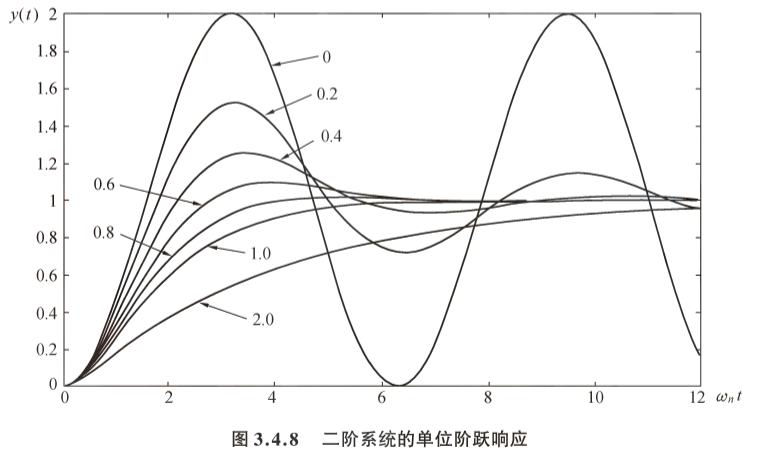
\includegraphics[width = .4\textwidth]{note/time-domain analysis/figure/4.png}
\end{center}

\subsection{二阶系统的单位冲激响应}
由已知其输出就等于系统的闭环传递函数：$Y(s) = \dfrac{\omega_n^2}{s^2 +2\zeta \omega_n s+\omega_n^2}$\\

对此式做Laplace反变换即可得到下列各种情况下的二阶系统单位冲激响应：
\begin{enumerate}
    \item 无阻尼$(\zeta = 0)$：$k(t) = \omega_n \sin\omega_n t \quad (t\geq 0)$ 
    \item 欠阻尼$(0<\zeta<1)$：$k(t) = \dfrac{\omega_n}{\sqrt{1-\zeta^2}}\sin \omega_d t \quad (t\geq 0 )$
    \item 临界阻尼$(\zeta = 1)$：$k(t) =  \omega_n^2 t e^{-\omega t} \quad(t\geq 0)$
    \item 过阻尼$(\zeta > 1)$：$k(t) = \dfrac{\omega_n}{2\sqrt{\zeta^2-1}}[e^{-(\zeta - \sqrt{\zeta^2 - 1})\omega_n t}-e^{-(\zeta + \sqrt{\zeta^2 - 1})\omega_n t}] \quad (t\geq 0)$ 
\end{enumerate}

用一个图可以一起表示上述四个情况的图像：
\begin{center}
    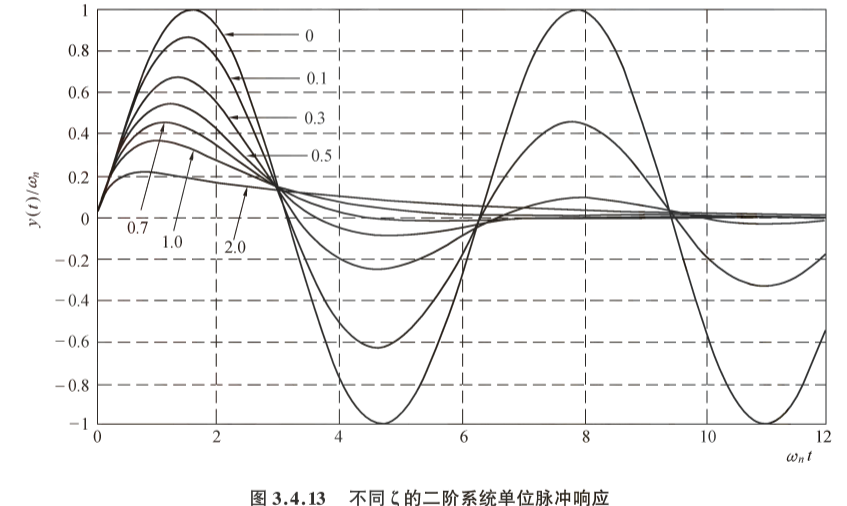
\includegraphics[width = .5\textwidth]{note/time-domain analysis/figure/5.png}
\end{center}

单独讨论二阶欠阻尼系统的单位冲激响应，如图所示：
\begin{center}
    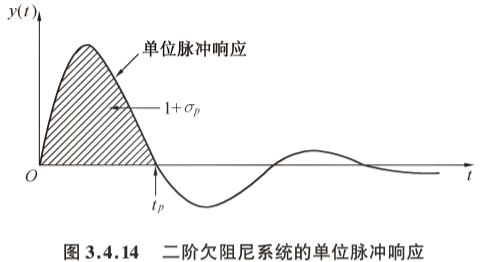
\includegraphics[width = .3\textwidth]{note/time-domain analysis/figure/6.png}
\end{center}
由于$\int_0^{t_p} k(t) dt = y(t_p) = 1+\sigma_p$，
所以上图中阴影部分面积为$1+\sigma_p$

\subsection{二阶系统的单位斜坡响应}
由已知可得系统在复频域的输出为：
\begin{equation*}
    Y(s) = \frac{\omega_n^2}{s^2+2\zeta \omega_n s+\omega_n^2}\cdot \frac{1}{s^2} = \frac{1}{s^2}-\frac{2\zeta/\omega_n}{s} + \frac{2\zeta(s+\zeta\omega_n)/\omega_n+(2\zeta^2 -1)}{s^2+2\zeta \omega_n s +\omega_n^2}
\end{equation*}

对此式做Laplace反变换即可得到下列各种情况下的二阶系统单位斜坡响应：
\begin{enumerate}
    \item 欠阻尼$(0<\zeta<1)$：$y(t) = t-\dfrac{2\zeta}{\omega_n} + \dfrac{1}{\omega_n\sqrt{1-\zeta^2}} e^{-\zeta\omega_n t}\sin (\omega_d t + \arctan\dfrac{2\zeta\sqrt{1-\zeta^2}}{2\zeta^2 - 1})$

    \item 临界阻尼$(\zeta =1)$：$y(t) = t - \frac{2}{\omega_n} + \frac{2}{\omega_n}e^{-\omega_n t}(1 + \dfrac{\omega_n}{2} t)$

    \item 过阻尼$(\zeta >1)$：$y(t) = t - \dfrac{2\zeta}{\omega_n} - \dfrac{2\zeta^2 - 1 - 2\zeta\sqrt{\zeta^2 - 1}}{2\omega_n \sqrt{\zeta^2 - 1}}e^{-(\zeta - \sqrt{\zeta^2 - 1})\omega_n t} + \dfrac{2\zeta^2 - 1 +2\zeta \sqrt{\zeta^2 - 1}}{2\omega_n \sqrt{\zeta^2 -1}}e^{-(\zeta - \sqrt{\zeta^2-1})\omega_n t}$
\end{enumerate}

\section{高阶系统的时域分析}
\subsection{高阶系统的阶跃响应}
高阶系统的闭环传递函数的一般形式是：
\begin{equation*}
    \varPhi (s) = \frac{Y(s)}{R(s)} = \frac{b_m s^m + b_{m-1} s^{m-1} + \cdots + b_1 s +b_0}{a_n s^n + a_{n-1} s^{n-1} + \cdots + a_1 s +a_0} = \frac{k\prod_{i=1}^m(s-z_i)}{\prod_{j=1}^n(s-s_j)}\text{(零极点形式)}
\end{equation*}

对上式运用Laplace反变换（参照定义1.3.2中Laplace逆变换的留数算法）

\subsection{闭环主导极点}
\begin{definition}[闭环主导极点]
    在高阶系统中存在很多极点，将对系统动态过程起主导作用的闭环极点，称为闭环主导极点
\end{definition}

寻找闭环主导极点的一种方法（不完全能用）：若在闭环极点中存在一对共轭复数极点（或一个实数极点）距离虚轴最近，其他极点到虚轴的距离都是它的5倍以上，并且距离虚轴较近处又没有单独的闭环零点，则这对或这个距离虚轴最近的极点称为高阶系统的主导极点

\section{改善控制系统动态性能的方法}
\subsection{速度反馈}
如图所示为带有速度反馈的二阶系统：
\begin{center}
    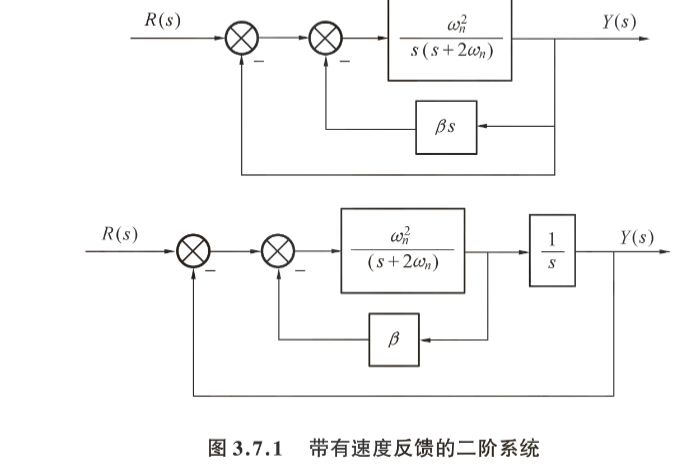
\includegraphics[width = .4\textwidth]{note/time-domain analysis/figure/7.png}
\end{center}

引入速度反馈后，系统的闭环传递函数为：
\begin{equation*}
    \varPhi(s) = \frac{Y(s)}{R(s)} = \frac{\omega_n^2}{s^2 + (2\zeta \omega_n + \omega_n^2 \beta)+\omega_n^2} = \frac{\omega_n^2}{s^2 + 2\overline{\zeta} \omega_n s + \omega_n^2}
\end{equation*}

显然，在引入速度反馈后，系统的阻尼比$\overline{\zeta}$要比原阻尼比$\zeta$要大
\begin{example}
    二阶系统的方框图如图所示，要求闭环系统的超调量$\sigma_p = 16.3\%$，峰值时间$t_p = 1$s，求放大器的放大倍数$K_0$和速度反馈系数$\tau$
    \begin{center}
        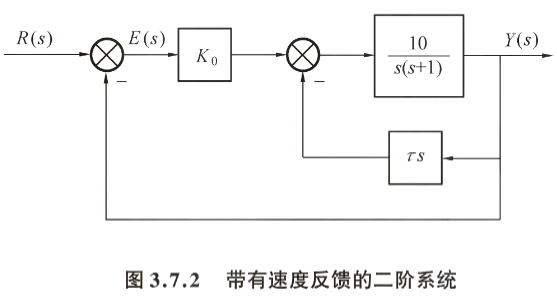
\includegraphics[width = .3\textwidth]{note/time-domain analysis/figure/8.png}
    \end{center}
    \textbf{解}：带有速度反馈系统的开环传递函数$G(s)$和闭环传递函数分别为：
    \begin{equation*}
        \begin{split}
            G(s) &= \frac{10K_0}{s^2 + (1+10\tau)s} \\
            \varPhi(s) &=\frac{10K_0}{s^2+(1+10\tau)s + 10K_0}
        \end{split}
    \end{equation*}

    由系统的闭环传递函数可以得出：
    \begin{equation*}
        \begin{split}
            \omega_n^2 &= 10K_0 \\
            2\zeta \omega_n &= 1+10\tau
        \end{split}
    \end{equation*}
    由已知可得：
    \begin{equation*}
        \begin{split}
            \sigma_p &= e^{-\zeta \pi /\sqrt{1-\zeta^2}}  = 0.163\\
            t_p/\mathrm{s} &= \frac{\pi}{\omega_n \sqrt{1-\zeta^2}} =1
        \end{split}
    \end{equation*}

    解得：$K_0 = 1.32,\tau = 0.263$
\end{example}

\subsection{PD控制}
如图所示为PD控制系统示意图：
\begin{center}
    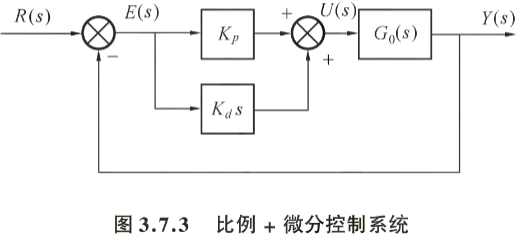
\includegraphics[width = .3\textwidth]{note/time-domain analysis/figure/9.png}
\end{center}

由图可知PD控制器的传递函数为：
\begin{equation*}
    G_c(s) = \frac{U(s)}{E(s)} = K_p + K_d s = K_p(1+\frac{K_d}{K_p}s) = K_p(1+\tau s)
\end{equation*}

下面以欠阻尼二阶系统为例讨论PD控制对改善系统动态过程的作用：
\begin{example}
    在图3.7.3中，设$G_0 (s) = \dfrac{K_0}{s(Ts+1)} $ 则：\\
    在没有PD校正的情况下，系统的闭环传递函数为：
    \begin{equation*}
        \varPhi(s) = \frac{K_0}{Ts^2+s+K_0}
    \end{equation*}

    此时$\omega_n = \sqrt{K_0/T},\zeta = 0.5 \sqrt{K_0 T}$\\

    采用PD校正后的传递函数为：
    \begin{equation*}
        \overline{\varPhi}(s) = \frac{K_0 K_p (\tau s + 1)}{Ts^2 + (K_0 K_p \tau+1)s + K_0 K_p}
    \end{equation*}

    此时相应的参数变化为：$\overline{\omega_n} = \sqrt{\dfrac{K_0 K_p}{T}} , \overline{\zeta} = \frac{K_0 K_p \tau +1}{2 \sqrt{T K_0 K_p}}$\\

    其中$\tau = \dfrac{K_d}{K_p}$

    对比前后参数的变化，可以看到：只要适当选取$K_p , K_d$的值，就可以增大系统无阻尼振荡频率和阻尼比，使系统的快速性和平稳性都得到改善。
\end{example}

